%!TEX root = main.tex


\chapter{Learning the lateral wavelength of Dutch railway vehicles by using the simulation results presented in D181 reports}\label{sec:wavelengthstudy}

As a conclusion in DT329 report, the lateral dynamic effects of railway vehicles are all wavelength phenomenon. The lateral wavelength of trains is a constant characteristics of themselves which doesn't change with outer environment. However, while the wavelength for axle repeat pattern is easy to get, the wavelength for kinematic movement normally requires heavy FEM simulations and post analysis of the response spectrum. 

Although it has been concluded in the previous chapter that avoiding resonance frequency is not a correct strategy for dynamics design in general, investigating the wavelength of trains can serve for the practical analysing methods that will be developed in following chapters in an alternative way.

This research aims to investigate both wavelength of trains running in the Netherlands. The axle repeat pattern wavelength is created by collecting all the possible axle layouts. The kinematic movement wavelength is created by developing a approximate methods that avoids heavy FEM simulations. 


\section{Effects investigated in wavelength study}

Effects investigated in this report will be the same effects investigated in DT 329, which is described in Sec.\ref{sec:resonance329}. However, according to the statement in Sec.2.3[Summary of results] in the same report,

\begin{quote}
Even when the axle repeat frequency matches the first lateral bending mode of each span, there is no evidence that the resonant behaviour of the span and train has any effect on subsequent spans, since the resonant effects do not appear to grow from span to span.
\end{quote}

the third investigated resonance effect 'coincidence between the length of the span and the kinematic wavelength of the trailing vehicles' is neglected in this thesis because it is concluded in \citet{d181dt329} that resonance do not grow from span to span. 


\section{Equivalent conicity used in this study}
According to \citet[Section.2.6]{esveld2001modern}, 

\begin{quote}
    Practical research has shown that over a period of time wheel profiles stabilise with wear at an equivalent conicity of 0.2 to 0.3. With regards to running stability, the equivalent conicity must remain below 0.4 and to ensure the centering effect it must be greater than 0.1.
\end{quote}

conicity range will be 0.2 to 0.3.

It is suggested by this report that vehicle maintenance sector ensure wheels of train wheels stay in the safe zone of conicity. 


\section{Study on wavelength of lateral kinematic movement}

The kinematic movement of the train on the rail is much similar to klingel movement. This section aims to assess the capability of using klingel formula to predict the wavelength of the whole train.

Klingel movement is proposed by Klingel which can well predict the moving trend of a single wheelset on a straight railway track. However, the kinematic movement of a certain wheelset assembled into a running train is different from the movement of a single free wheelset. This is due to multiple bodies interact with each other, introducing more complicated mechanism in wheel/rail interaction. 

This  study focuses on Klingel movement of a bogie. First part of the  study will try to discuss the relationship of Klingle frequency of a wheelset and kinematic movement frequency of a whole train. Second part of the study will use realistic data of Dutch railway/vehilces to assess the frequency bandwidth of Dutch native trains.

This section will include following parameters to be studied:

\begin{enumerate}[-]
	\item Speed of train, radius of the wheel and conicity of the wheel. 
	\item Gauge distance is fixed to 1435mm according to UIC standard. 
	\item Frequency is linear to speed if other parameters are fixed.
\end{enumerate}


\subsection{Comparison between Klingle movement and train kinematic movement studied in D181 DT329}

In this section the kinematic wave length of trains used in D181 VAMPIRE simulations will be calculated by klingel's formula and compared with the wavelength value obtained in VAPIRE simulation.

Klingel's formula:
Klingel has done experiments and has given that the wavelength of a single wheelset:

$$ \lambda_0 = 2 \pi \sqrt{\frac{rG}{2\gamma} }$$

where:

G = Dynamic Gauge

r = Dynamic Wheels Radius

g = Conicity

For 2 wheelsets connected by a bogie:

$$ \lambda = \lambda_0 \sqrt{1+(\frac{I}{G})^2}  $$

where:

I = Rigid wheel base

By inputting the related train parameters used in VAMPIRE simulations into the Klingel formula, following table is obtained.

\begin{table}[h]
  \centering
  \caption{Approxiamte letaral kinematic wavelength calcualted by improved Klingel formula}
    \begin{tabular}{cccccccccccccccc}
    \toprule
    & Gauge & BWD & Radius & Conicity & Wavelength($\lambda_0$) &Wavelength($\lambda$) & \\
    \midrule
    BR CLASS 56 LOCO  & 1435 & 4180 & 290 & 0.05 & 12.8175 & 39.4750 \\
    FS E444 LOCO  & 1435 & 2600 & 550 & 0.05 & 17.6517 & 36.5301 \\
    FS ETR500 LOCO  & 1435 & 3000 & 550 & 0.05 & 17.6517 & 40.9070\\
    UIC FREIGHT WAGON  & 1435 & 0 & 460 & 0.05 & 16.1430 & 16.1430 \\
    FS ETR500 COACH  & 1435 & 3000 & 440 & 0.05 & 15.7882 & 36.5883 & \\
    UIC COACH  & 1435 & 2560 & 445 & 0.05 & 15.8776 & 32.4718 &  \\
    \bottomrule
    \end{tabular}%
  \label{tab:wavelengthkinematic}%
\end{table}%


By comparing the result from Table.\ref{tab:wavelengthkinematic} and kinematic wavelength obtained by D181, extracted as Table.\ref{tab:329kinematicwavelength}, parametric study results show close prediction for kinematic wavelength of freight train locomotive/coach/wagon. It's because freight train suspension system is simpler and stiffer compared to passenger train's, making the behaviour of train acts more similar to the behaviour of a single wheelset of bigger mass. 


Wavelength for UIC freight wagon is a special case and it's not meeting the wavelength results in VAMPIRE simulations. This is probably because this car has a different design. It can be seen from in Figure.\ref{fig:uicoach} that only 2 axles are installed and there's no wagon installed. See Figure.\ref{fig:2axlefreight} and Figure.\ref{fig:4axlefreight} for their different axle configurations.

\begin{figure}[h]
	\centering
	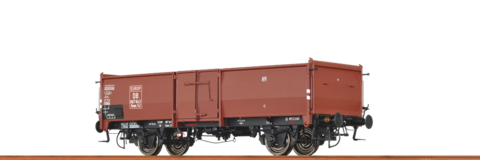
\includegraphics[width=0.5\textwidth]{2alxefreight.png}
	\caption{Example of a 2-axle freight wagon}
	\label{fig:2axlefreight}
\end{figure}

\begin{figure}[h]
	\centering
	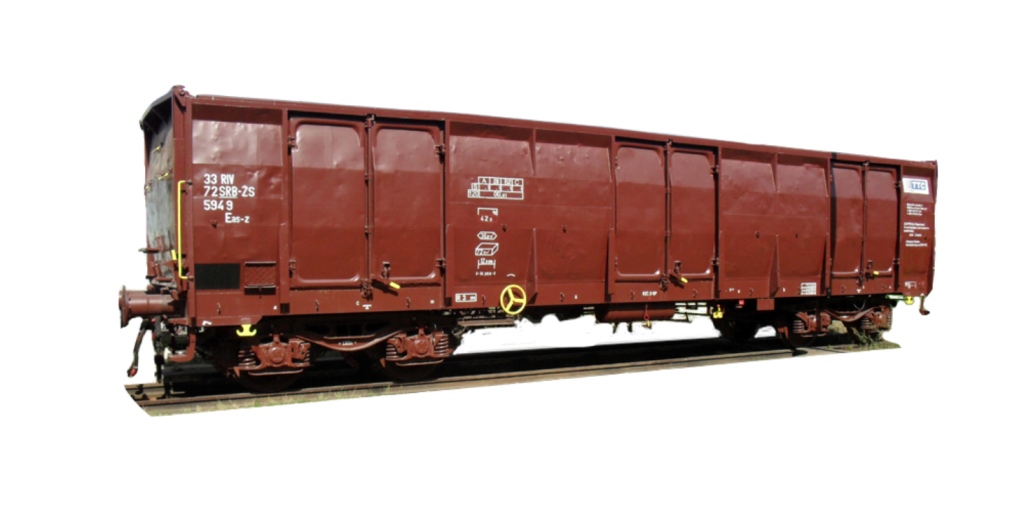
\includegraphics[width=0.5\textwidth]{4alxefreight.png}
	\caption{Example of a 4-axle freight wagon}
	\label{fig:4axlefreight}
\end{figure}


The train parameter used in this part of parametric study is attached in the Appendix.\ref{app:mu}. 


\section{Assess of wavelength bandwidth based on realistic data of Dutch Rail/Vehicle}

The wavelength of passenger coach is highly related to the characteristics of its suspension systems. These data are often difficult to obtain. Since the improved Klingel formula ignored the effect of suspension system, the results in this section is only approximate value for the wavelength of kinematic movement.


Future research is highly recommended to be conducted to study the kinematic wavelength of complete vehicles in the Netherlands, using realistic data of their suspension systems.


Table.\ref{tab:wavelengthrealistic} is created by processing Dutch wheel radius and wheelbase data collected from document\citet{trainparameters}. 
Thus range of $\lambda$ is obtained by inputting realistic data in Kingel formula, illustrated in Table.\ref{tab:wavelengthrealistic}.

\begin{table}[h]
  \centering
  \caption{Wavelength of kinematic movement generated by realistic value}
    \begin{tabular}{cccccccccccccccc}
    \toprule
    & Gauge & BWD & Radius & Conicity & Wavelength\_0() &Wavelength & \\
    \midrule
    \textbf{Freight 2-axle} & 1435 & 0 & 500 & 0.05 & 16.8303 & 16.8303 \\
    \textbf{} & 1435 & 0 & 500 & 0.2 & 8.4151 & 8.4151  \\
    \textbf{} & 1435 & 0 & 500 & 0.3 & 6.8709 & 6.8709  \\
    \textbf{}       &       &       &       &       &       &       &  \\
    \textbf{Freight 4-axle} & 1435 & 1800 & 500 & 0.05 & 16.8303 & 26.9988 \\
    \textbf{} & 1435 & 1800 & 500 & 0.2 & 8.4151 & 13.4994  \\
    \textbf{} & 1435 & 1800 & 500 & 0.3 & 6.8709 & 11.0222  \\
    \textbf{}       &       &       &       &       &       &       &  \\
    \textbf{Passenger} & 1435 & 2500 & 460 & 0.05 & 16.1430 & 32.4275 \\
    \textbf{} & 1435 & 2500 & 460 & 0.2 & 8.0715 & 16.2137  \\
    \textbf{} & 1435 & 2500 & 460 & 0.3 & 6.5904 & 13.2385 \\
    \textbf{}       &       &       &       &       &       &       &  \\
    \textbf{} & 1435 & 2750 & 460 & 0.05 & 16.1430 & 34.8947 \\
    \textbf{} & 1435 & 2750 & 460 & 0.2 & 8.0715 & 17.4473  \\
    \textbf{} & 1435 & 2750 & 460 & 0.3 & 6.5904 & 14.2457  \\
    \textbf{}       &       &       &       &       &       &       &  \\
    \textbf{Locomotive} & 1435 & 2400 & 500 & 0.05 & 16.8303 & 32.7960 \\
    \textbf{} & 1435 & 2400 & 500 & 0.2 & 8.4151 & 16.3980  \\
    \textbf{} & 1435 & 2400 & 500 & 0.3 & 6.8709 & 13.3889  \\
    \textbf{}       &       &       &       &       &       &       &  \\
    \textbf{} & 1435 & 2950 & 500 & 0.05 & 16.8303 & 38.4751 \\
    \textbf{} & 1435 & 2950 & 500 & 0.2 & 8.4151 & 19.2376  \\
    \textbf{} & 1435 & 2950 & 500 & 0.3 & 6.8709 & 15.7074  \\
    \bottomrule
    \end{tabular}%
  \label{tab:wavelengthrealistic}%
\end{table}%

For conservative usage, please take the value yielded by 0.3 wheel conicity. However, as proved in previous section, this estimation is in closest estimation of simulation results when concity is 0.05.

% Figure.\ref{fig:wavelengthkinematicfreight} and Figure.\ref{fig:wavelengthkinematicpass} are generated according to linear relationship between frequency and speed, using the wavelength $\lambda$ obtained in Table.\ref{tab:wavelengthrealistic}:

% $$ f = v \frac{1}{\lambda} $$


% \begin{figure}[h!]
% \centering
% \begin{tikzpicture}[trim axis left, trim axis right]
% \begin{axis}[
%     xlabel={$v(m/s)$},
%     ylabel={$f(Hz)$},
%     ymin = 0, xmin = 0, xmax = 44.4,
%     legend entries={$\sfrac{1}{\lambda}=0.059$,$\sfrac{1}{\lambda} =0.072$,$v=33.3 m/s$,$f=0.3Hz$},
%     grid = both,
%     minor y tick num= 4,
%     minor x tick num= 4,
%     legend pos = north west,
% ]
% \addplot[blue, domain = 0:44.4,samples=201,name path = A]{0.059*x};
% \addplot[red, domain = 0:44.4,samples=201, name path = B]{0.072*x};
% \addplot[mark=none, dashed]  coordinates {(33.3,0) (33.3,5) };
% \addplot[domain = 0:44.4,samples=10,dashed]{0.3};
% \addplot[gray] fill between[of=A and B];
% \end{axis}
% \end{tikzpicture}
% \caption{Lateral frequency of freight train with respect to speed(Kinematic movement)}
% \label{fig:wavelengthkinematicfreight}
% \end{figure}

% \begin{figure}[h!]
% \centering
% \begin{tikzpicture}[trim axis left, trim axis right]
% \begin{axis}[
%     xlabel={$v(m/s)$},
%     ylabel={$f(Hz)$},
%     ymin = 0, xmin = 0, xmax = 44.4,
%     legend entries={$\sfrac{1}{\lambda}=0.062$,$\sfrac{1}{\lambda}=0.076$,$v=33.3 m/s$,$f=0.3Hz$},
%     grid = both,
%     minor y tick num= 4,
%     minor x tick num= 4,
%     legend pos = north west,
% ]
% \addplot[blue, domain = 0:44.4,samples=201, name path = A]{0.062*x};
% \addplot[red, domain = 0:44.4,samples=201, name path = B]{0.076*x};
% \addplot[mark=none,dashed]  coordinates {(33.3,0) (33.3,3.5) };
% \addplot[domain = 0:44.4,samples=10,dashed]{0.3};
% \addplot[gray] fill between[of=A and B];
% \end{axis}
% \end{tikzpicture}
% \caption{Lateral frequency of passenger train with respect to speed(Kinematic movement)}
% \label{fig:wavelengthkinematicpass}
% \end{figure}

\section{Lateral wavelength of axle repeat pattern of Dutch Railway Vehicles}

This section will generate lateral wavelength value of axle repeat pattern of Dutch Railway Vehicles. Although DT329 provided wavelength values for some trains in Table.\ref{tab:329axlerepeat} but the way of obtaining these values was not mentioned. So an interpretation is needed to understand how to obtain the axle repeat pattern wavelength.

By observing Table.\ref{tab:329axlerepeat}, it can be seen that axle spacing layout is the only raw data needed to generate axle repeat pattern wavelength. The value is regardless of all other parameters. There are several axle space combinations in the table, but only one combination was finally put emphasis on during the analysis phase of axle repeat resonance research. They are

\begin{enumerate}[-]
    \item \textit{'wagon n axle m - wagon n+1 axle m'} for freight train, 
    \item \textit{'coach n axle m - coach n+1 axle m'} for passenger train,
    \item \textit{'coach n axle m - coach n+1 axle m'} for high speed train.
\end{enumerate}

It's still hard to comprehend above combinations so further interpretation is done by comparing it to train parameters in Appendix.\ref{app:dt329data}. It is found 

By comparing Fig.\ref{fig:trainparameters} and Table.\ref{tab:329axlerepeat}. It can be seen that 'wagon n axle m - wagon n+1 axle m' means the distance between one axle in the previous car and another axle in next car in the same location. The same goes for passenger train and high speed train. To better understand this spacing, please see L\_Coa in Figure.\ref{fig:trainparameters}. 

\begin{table}[h!]
  \centering
  \caption{Wavelength of axle repeat pattern($m$)}
    \begin{tabular}{rrrrrrrrr}
    \toprule
    \textbf{Type} & \textbf{L\_coa min} & \textbf{L\_coa max} & \textbf{2*L\_coa min } & \textbf{2*L\_coa max} \\
    \midrule
    \textbf{CB\_1} & 23.8  & 25.3  & 47.6  & 50.6 \\
    \textbf{CB\_2} & 25.3  & 27.5  & 50.6  & 55    \\
    \textbf{AB\_1} & 14.9  & 16    & 29.8  & 32     \\
    \textbf{AB\_2} & 18.8  & 19.5  & 37.6  & 39    \\
    \textbf{AB\_3} & 17    & 17.5  & 34    & 35   \\
    \textbf{AB\_4} & 18.7  & 19.2  & 37.4  & 38.4  \\
    \textbf{SA\_1} & 9.2   & 9.8   & 18.4  & 19.6  \\
    \textbf{SA\_2} & 12.8  & 13.5  & 25.6  & 27    \\

    \bottomrule
    \end{tabular}%
  \label{tab:wavelengthaxlerepeat}%
\end{table}%

Lateral wavelength of axle repeat pattern is then obtained by extracting all possible L\_Coa values from MU standards in \citet{EC15528}, illustrated in Table.\ref{tab:wavelengthaxlerepeat}. Detailed information about MU classes can be found in Appendix.\ref{app:mu}.


After examing the content in analysing section of DT329 resonance study, it is found that double length of L\_Coa is not taken into account in analysis phase. This means although D181 committee calculated double length of L\_Coa, these values were never used. Thus it is advisable for the usage of lateral axle repeat pattern wavelength, extracting only L\_Coa min column and L\_Coa max column.


% \begin{figure}[h!]
% \centering
% \begin{tikzpicture} 
%     \begin{axis}[
%     xlabel={$v(m/s)$},
%     ylabel={$f(Hz)$},
%     ymin = 0, xmin = 0, xmax = 44.4,
%     %legend entries={$i=0.057$,$i=0.07$,$v=33.3 m/s$,$f=0.3Hz$},
%     grid = both,
%     minor y tick num= 4,
%     minor x tick num= 4,
%     ]
%     \addplot[blue,name path=A,domain=0:44.4] {0.036*x};
%     \addplot[red, name path=B,domain=0:44.4] {0.042*x};
%     \addplot[black] fill between[of=A and B];
%     \addplot[blue,name path=C,domain=0:44.4] {0.051*x};
%     \addplot[red, name path=D,domain=0:44.4] {0.053*x};
%     \addplot[black] fill between[of=C and D];
%     \addplot[blue,name path=E,domain=0:44.4] {0.057*x};
%     \addplot[red, name path=F,domain=0:44.4] {0.059*x};
%     \addplot[black] fill between[of=E and F];
%     \addplot[blue,name path=G,domain=0:44.4] {0.063*x};
%     \addplot[red, name path=H,domain=0:44.4] {0.067*x};
%     \addplot[black] fill between[of=G and H];
%     \addplot[blue,name path=I,domain=0:44.4] {0.074*x};
%     \addplot[red, name path=J,domain=0:44.4] {0.078*x};
%     \addplot[black] fill between[of=I and J];
%     \addplot[blue,name path=K,domain=0:44.4] {0.102*x};
%     \addplot[red, name path=L,domain=0:44.4] {0.109*x};
%     \addplot[black] fill between[of=K and L];
%     \addplot[blue,name path=M,domain=0:44.4] {0.018*x};
%     \addplot[red, name path=N,domain=0:44.4] {0.021*x};
%     \addplot[gray] fill between[of=M and N];
%     \addplot[blue,name path=O,domain=0:44.4] {0.026*x};
%     \addplot[red, name path=P,domain=0:44.4] {0.027*x};
%     \addplot[gray] fill between[of=O and P];
%     \addplot[blue,name path=Q,domain=0:44.4] {0.029*x};
%     \addplot[red, name path=R,domain=0:44.4] {0.029*x};
%     \addplot[gray] fill between[of=Q and R];
%     \addplot[blue,name path=S,domain=0:44.4] {0.031*x};
%     \addplot[red, name path=T,domain=0:44.4] {0.034*x};
%     \addplot[gray] fill between[of=S and T];
%     \addplot[blue,name path=U,domain=0:44.4] {0.037*x};
%     \addplot[red, name path=V,domain=0:44.4] {0.039*x};
%     \addplot[gray] fill between[of=U and V];
%     \addplot[blue,name path=W,domain=0:44.4] {0.051*x};
%     \addplot[red, name path=X,domain=0:44.4] {0.054*x};
%     \addplot[gray] fill between[of=W and X];
%     \addplot[dashed,thick,red, domain=0:44.4] {0.3};
% \end{axis}
% \end{tikzpicture}
% \caption{Two repeat pattern frequencies with respect to speed}
% \label{fig:repeatpatternfrequencies}
% \end{figure}

\section{Conclusion of wavelength study}

The lateral resonance effects between running train and railway bridge include two phenomenon: Axle repeat pattern and Kinematic movement. Those two phenomenon are all wavelength phenomenon, which means for every specific train, the wavelength of its axle repeat pattern and kinematic movement remains constant. In other word, the frequency of lateral dynamic effect caused by the operating of trains on bridge is directly related to the speed.

Since the wavelength for the two phenomenon on the same train are not likely to be equal, the possible range of wavelength for both phenomenon were investigated in this chapter. The possible axle repeat pattern wavelength is approximately 10m-30m covering all train types and kinematic wavelength is 13m to 17m covering all train types. It can be seen that axle repeat pattern possess a broader range of wavelength than kinematic movement.

It also can be concluded that for any railway bridge, resonance between the bridge itself and train can happen if the train is running at a corresponding resonance speed according to its wavelength. So avoiding resonance is not a valid strategy to choose, not to mention the apparent frequency shift phenomenon to be discussed in Chapter.\ref{sec:resonance329}. 

To be noted that these wavelength are also not the exact wavelength in real-life scenario but an estimation, especially for kinematic movement. But it gave away a rough idea about the magnitude of trains' wavelength, and, can be used for practical design purposes. To see the usage of studied wavelength, please see Chapter.\ref{sec:parcticalmethod}.

\chapter{Development of new practical method for checking lateral resonance response of railway bridges based on VAMPIRE simulation results }\label{sec:parcticalmethod}

\section{Introduction}

This chapter proposes a new method for checking lateral resonance response of railway bridges. This method aims to provide an engineering solution for checking the deflection and acceleration of railway bridges when resonance happens under horizontal dynamic train load. Both creation and verification of the method is based on VAMPIRE simulation results provided in DT329 research.

The method features the combined usage of a simplified analytical structural model and a more refined lateral force model. The analytical structure model simulates a perfect resonance scenario for railway bridge. And the refined load model, which is a concentrated harmonic moving load, represents the lateral dynamic effects that occur because of the passing of the train. The combination of these two analytical elements will generate a resonance response conservative compared to the simulation output in DT329 because various types of disturbance were included in these simulation runs.

The analytical structural model that was introduced in Appendix.\ref{sec:analyticalmodel} and its explicit solution has already been worked out in the same chapter. Thus the main objective of this chapter is finding a better lateral force load model because current existing ones are too conservative(see Section.\ref{sec:refinedloadmodel}). The refined load model shall be able to be adopted universally for all regular train types. Once this load model is obtained and verified, it is then possible to take advantage of the combination of the load model and analytical solution for practical designing purposes.

\section{Overview of this chapter}

To give a clear overview of this chapter, procedure of development of the method  as following:

\begin{enumerate}
    \item \textit{Developing:} Develop a more practical load model to be used in pair with the analytical model introduced in previous chapter based on the VAMPIRE simulation outputs. See Section.\ref{sec:refinedloadmodel}
        \begin{enumerate}[label*=\arabic*.]
            \item Overview of both VAMPIRE numerical simulation method and analytical method. See Section.\ref{sec:overviewvampireanalytical}
            \item Find the analytical equivalent nosing forces amplitude for freight trains in 3 different cases presented in DT329 resonance research simulation. See Section.\ref{sec:findingequivalentamplitude}
            \item Find regular pattern and key parameter for the magnitude of nosing forces amplitude for freight trains. See Section.\ref{sec:keyparameterforequivalentamplitudeandhypothesis}
            \item Develop a conservative load model based on observed pattern of nosing force of freight trains. See Section.\ref{sec:keyparameterforequivalentamplitudeandhypothesis}
        \end{enumerate} 
    \item \textit{Verifying:} Validate the feasibility of combined usage of conservative load model and analytical model
        % \begin{enumerate}[label*=\arabic*.]
        %     \item What 
        % \end{enumerate}
    \item \textit{Finalizing:} Illustrate the usage of the method by applying it on a real railway bridge
\end{enumerate}

\begin{figure}[h!]
\centering
\begin{tikzpicture}[node distance=1cm, auto,]
    \node[punkt] (set1) {VAMPIRE simulation results inventory 1};
    \node[punkt, inner sep=15pt,right=2cm of set1]
        (am) {Analytical Method:Explicit solution and equivalent load amplitude};
    \node[punkt, right=2cm of am] (set2) {VAMPIRE simulation results inventory 2};
    \draw[->] (set1) to (am);
    \draw[->] (am) to (set2);
    \node[right=0.8cm of set1] (dummy1) {};
    \node[above=0.1cm of dummy1] (creation) {creation};
    \node[right=0.9cm of am] (dummy2) {};
    \node[above=0.1cm of dummy2] (verification) {verification};
\end{tikzpicture}
\caption{Workflow of the creation of analytical method}
\label{fig:workflowanalyticalmethod}
\end{figure}

\section{Development of refined load model}\label{sec:refinedloadmodel}

The load model provided in EN1991-2(nosing force) and D181 RP6(proposed criteria) are too conservative for dynamic analysis. The reason is that these forces are obtained by simulations ran on poorest maintained tracks with $7mm$ track irregularity standard deviation. In fact tracks are allowed to have lateral irregularities up to $1.8mm$ according to EN13848(Section.\ref{sec:lateraltrackirrgularities}). So existing lateral force models are enormous compared to real-life scenario. 

In addition, the existing load models are representative for hunting effects\citet[Proposed criteria]{d181}. However, according to \citet{majka2008effects}, although affected by varies parameters, critical speed for hunting effect is normally at 120km/h for modern railway vehicle and tracks. So at least for trains running slower than 120km/h, it can be conclude that hunting is not occurring. And their lateral force should be much less than the force magnitude mentioned in either EN1991-2 or D181 RP6.

Thus these existing load models are too big and not suitable for the analytical solution. A more precise load model is needed for coupled usage for analytical solution.

\subsection{Overview of VAMPIRE numerical simulation method and analytical method}\label{sec:overviewvampireanalytical}

The analytical model itself and its explicit expression have already been introduced and described in previous chapter. This section will give a overview on the input parameters of both VAMPIRE simulation and analytical model. This is not only due to the fact that VAMPIRE simulation was proved by D181 committee to be in close prediction with situ measurements, but also because in following sections VAMPIRE simulation results will be used as benchmark data for the development of analytical model's pairing load model. 

\begin{table}[h!]
    \centering
    \caption{Comparison between input parameters of DT329 VAMPIRE simulations and analytical model}
    \begin{tabular}{c|cc}
        \hline
        & Simulation & Analytical model \\
        \hline
        Bridge structure & simply supported beam & simply supported beam \\
        Span & Yes & Yes \\
        Stiffness & Yes & Yes \\
        Mass & Yes & Yes \\
        Damping & Yes & Yes \\
        Train & complete train as mass spring system & single moving harmonic load \\
        Train Speed & Yes & Yes \\
        Track irregularities & Yes & No \\
        Wheel profile & Yes & No \\
        Wheel-rail interaction & Yes & No \\
        \hline
    \end{tabular}
    \label{tab:comparisonsimulationanalytical}
\end{table}

As demonstrated in Table.\ref{tab:comparisonsimulationanalytical}, while input parameters for simulation are complicated, analytical model possesses less input parameters. 

That table shows that the single moving harmonic load in analytical model shall be capable of providing dynamic effect caused by train speed, track irregularities, wheel profile and wheel-rail interaction to the analytical model. Correct single moving harmonic load input shall yield the same result as VAMPIRE simulation provided that same span, stiffness, mass and damping value are adopted in both two calculating methods.

Thus finding the correct expression for the harmonic moving force is vital to the analytical model. The harmonic moving force has 3 parameters: speed $c$, frequency $\Omega$  and amplitude $Q$. Since speed $c$ simply equals to train speed and frequency $\Omega$ equals to the first natural bending frequency of the beam $\omega_1$, the amplitude of the harmonic force remains to be researched. Further development of the amplitude expression will be discussed in following sections.



\subsection{Finding equivalent lateral force amplitude for specific cases}\label{sec:findingequivalentamplitude}
In this section, equivalent lateral force amplitudes for the analytical solution are obtained. The equivalent lateral force amplitude does not represent real force magnitude in rail/wheel interaction, but a force amplitude that yields same result as VAMPIRE simulations using same input parameters if substituted into analytical solution. So this lateral force amplitude may not be correct if adopted in other structure models. On the other hand, analytical solution may yield imprecise results if not substituted with this exact equivalent force amplitude. They can only be used in pair with each other.

Thus in order to perform the comparison mentioned above, both input and output data of DT 329 VAMPIRE simulations are selected as reference data. The input data will be substituted into analytical model and the output data of VAMPIRE simulation will be compared with output of analytical model. 

3 sets of reference data are extracted from DT329 report. They are C1,C3,C9 in Figure.\ref{fig:c1},\ref{fig:c3} and \ref{fig:c9} respectively. These data are all extracted from resonance study so they are qualified to be used as reference data. Please note that C1,C3,C9 were all done on freight trains on same track sample. Finally 3 equivalent forces are collected from these 3 test samples to see regular pattern and relevant parameters for freight trains.

\begin{figure}[h!]
    \centering
    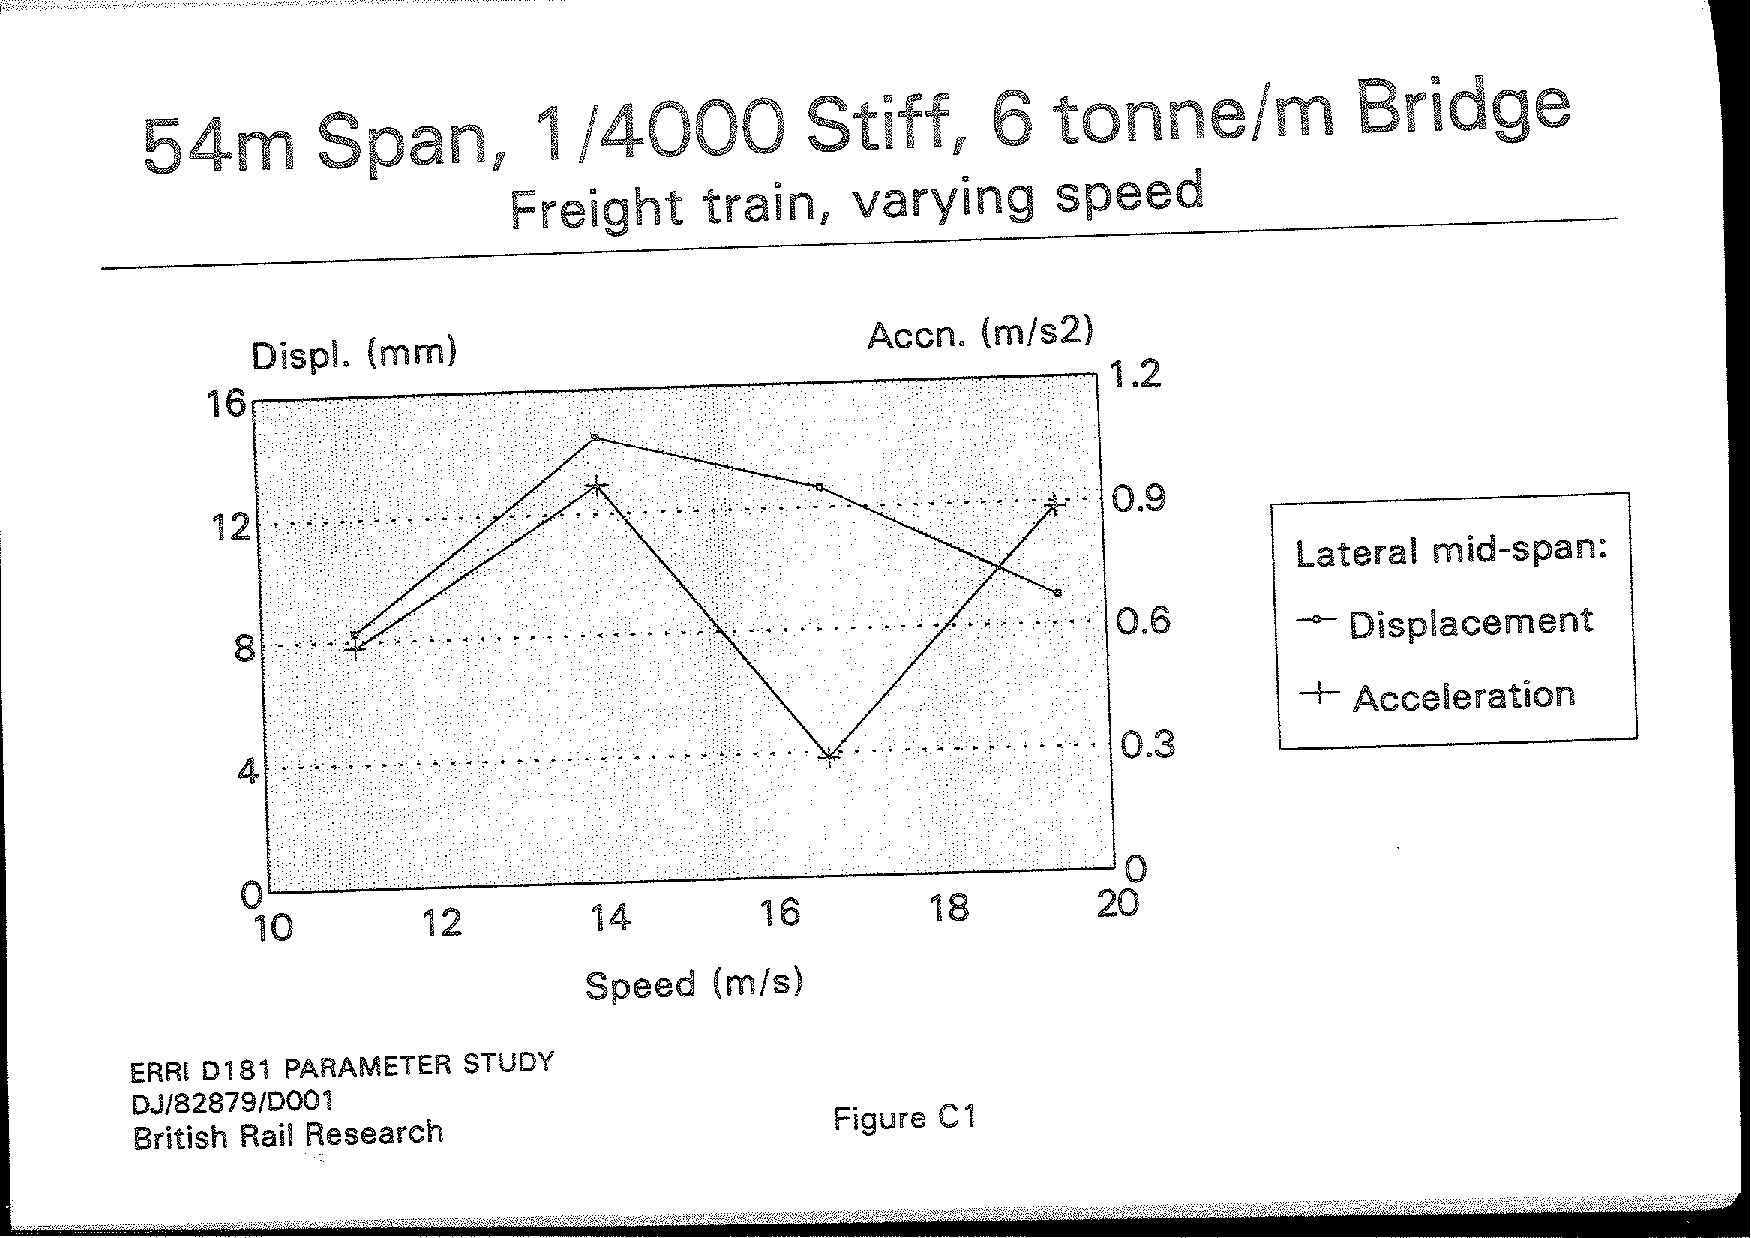
\includegraphics[width=0.8\textwidth]{c1}
    \caption{Figure C1 extracted from \citet{d181dt329} }
    % \label{fig:c1}
\end{figure}

\begin{figure}[h!]
    \centering
    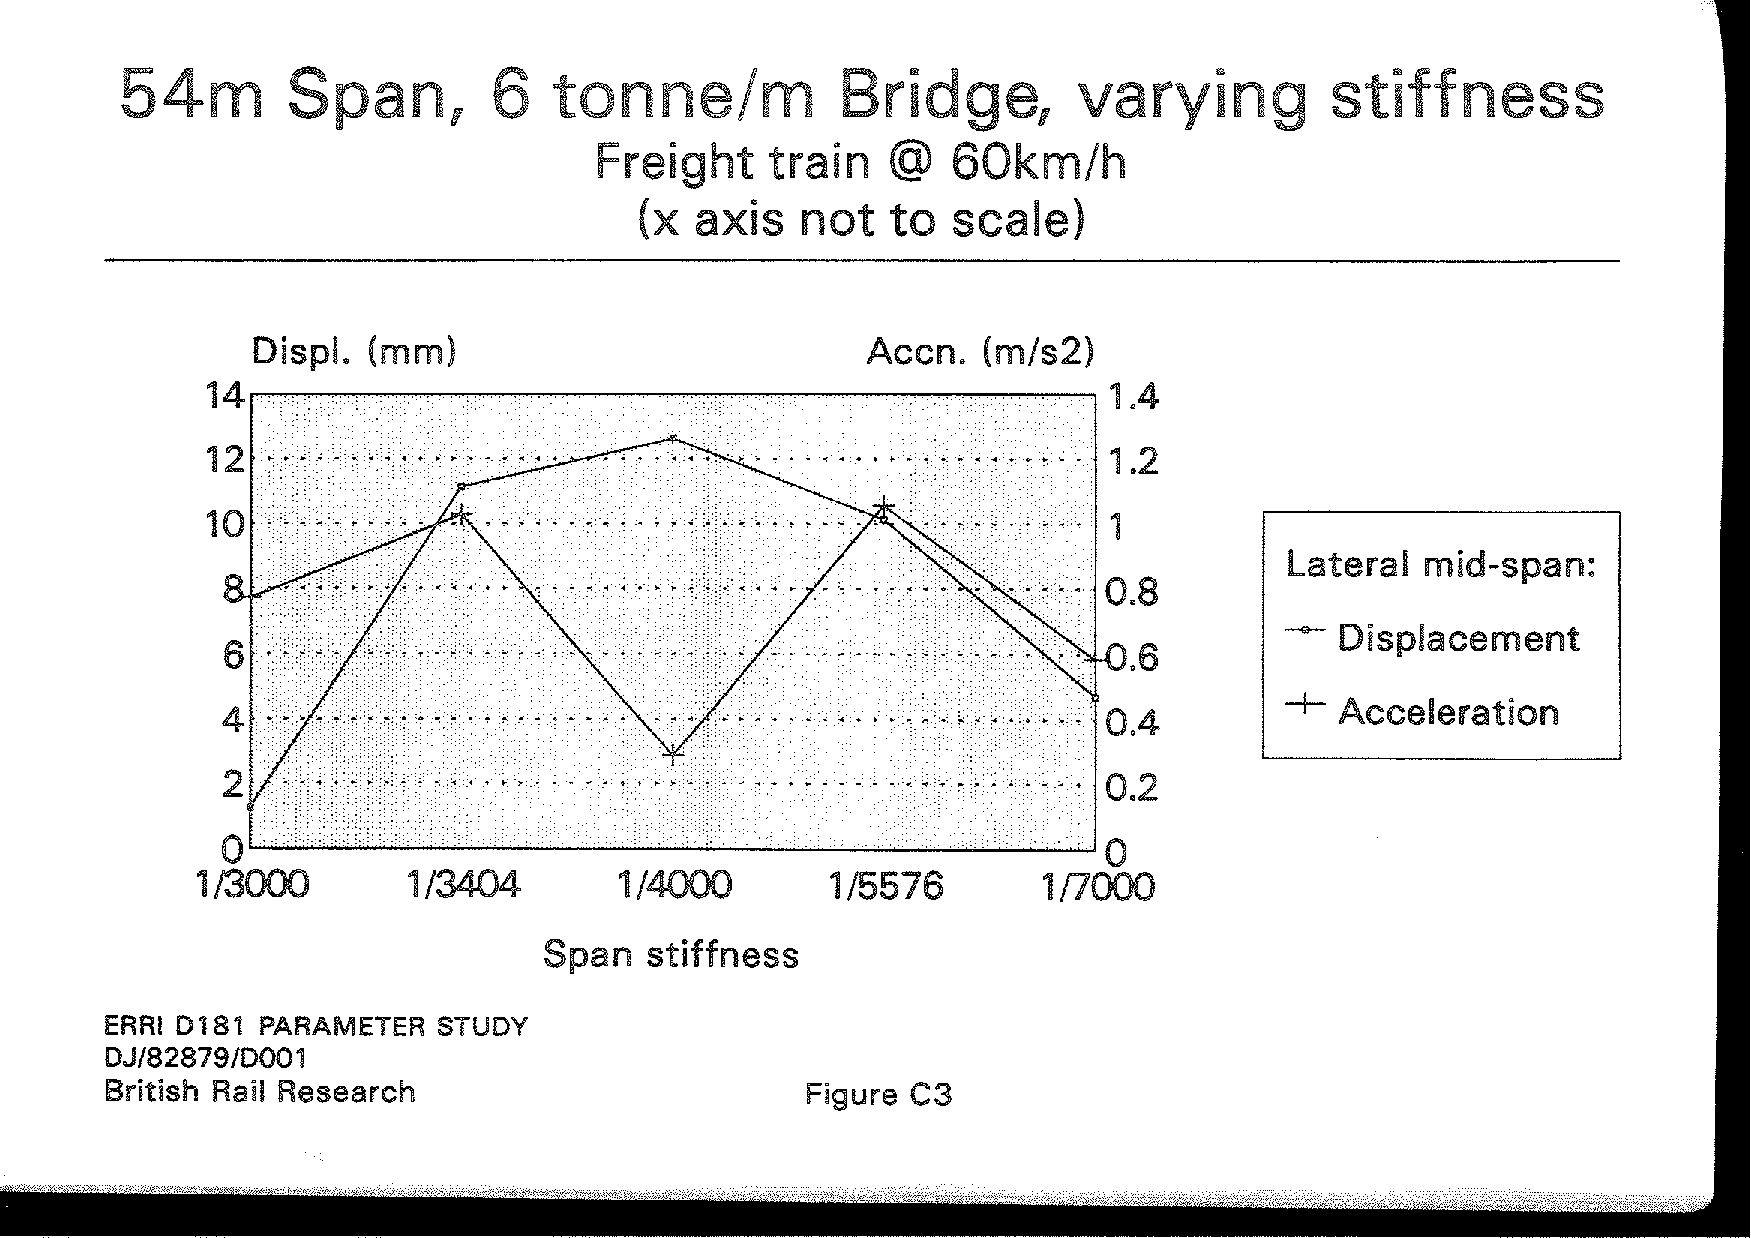
\includegraphics[width=0.8\textwidth]{c3}
    \caption{Figure C3 extracted from \citet{d181dt329} }
    % \label{fig:c3}
\end{figure}

\begin{figure}[h!]
    \centering
    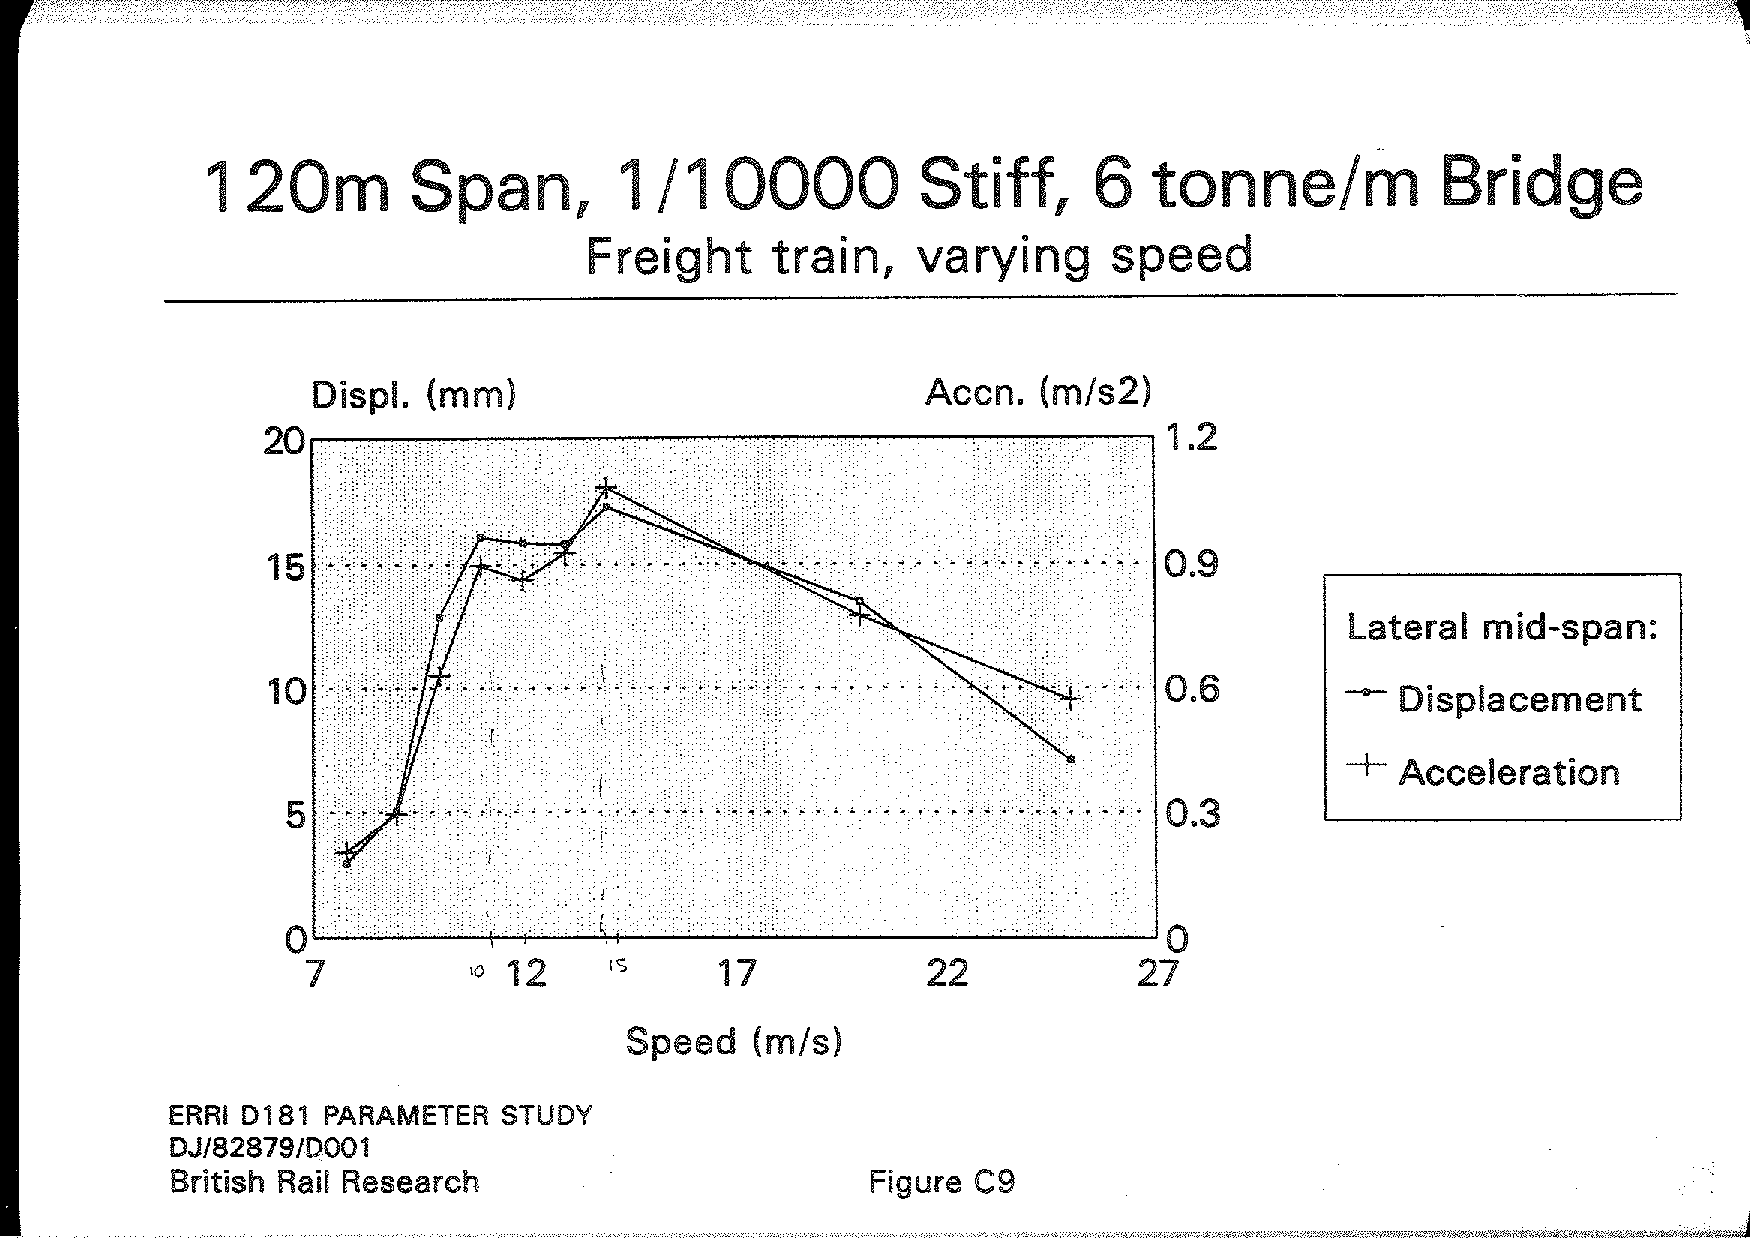
\includegraphics[width=0.8\textwidth]{c9}
    \caption{Figure C9 extracted from \citet{d181dt329} }
    % \label{fig:c9}
\end{figure}

By observing Eq.\ref{eq:v(x,t)simpleharmonic}, it is concluded that force amplitude is an independent variable and perfectly linear to the analytical output. Thus the equivalent force is obtained by inputing bridge parameters and train speed into the analytical solution Eq.\ref{eq:v(x,t)simpleharmonic} and manually increasing the force amplitude little by little until the peak response output reaches the same magnitude of peak simulation output. The parameters used and their corresponding results are presented in Table.\ref{tab:parametersetupsandequivalentforce}.


\begin{table}[h!]
    \centering
    \caption{Parameter setups and equivalent force amplitude for C1,C3,C9}
    \begin{tabular}{c|ccc}
        \hline
        & C1 & C3 & C9 \\
        \hline
        Stiffness($\sfrac{\delta_0}{l}$) & 1/4000 & 1/4000 & 1/10000 \\
        Span($m$) & 54m & 54 & 120 \\ 
        Mass per unit length($kg/m$) & 6000 & 6000 & 6000\\
        Speed of train($m/s$) & 14 & 16.67(60km/h) & 14\\
        Damping ratio & 1\% & 1\% & 1\%\\
        Train type & Freight & Freight & Freight \\
        Track & Coupled freight track & Coupled freight track & Coupled freight track \\
        \hline
        Equivalent load amplitude(kN) & 14 & 15 & 14 \\
        \hline
    \end{tabular}
    % \label{tab:parametersetupsandequivalentforce}
\end{table}

\subsection{Key parameter for equivalent force amplitude and hypothesis expression for refined load model}\label{sec:keyparameterforequivalentamplitudeandhypothesis}

By observing the equivalent load amplitude illustrated in Table.\ref{tab:parametersetupsandequivalentforce}, it is found that the equivalent load amplitude yielded by analytical solution meets the general principle of lateral track force concluded by DT329 track quality research. The general principle is that the lateral force is only relevant to speed if track quality and wheel conicity are fixed. And lateral force is irrelevant to the bridge parameters.
 
Because equivalent force amplitude meets the general lateral force principle, it is further expected that the equivalent force amplitude also has a similar form of force-speed relationship of DT329 VAMPIRE simulations. Due to the lack of reference data, it is impossible to make a reliable regression. Only a hypothesis expression can be created by scaling Eq.\ref{for:regressionfreight} to 14kN at 14m/s(reference data set C1). Please note only C1 was used in creating the hypothesis expression so C3 and C9 remains available for the verification.

\begin{equation}
    Q= 1928\times c^{0.7495}
\end{equation}

where:

$Q$: equivalent force amplitude($N$)

$c$: speed of the train($m/s$)

This scaling is reasonable because: according to the conclusion of DT329 track quality research, lateral forces generated on 7mm standard deviation tracks has a certain relationship with speed(Eq.\ref{for:regressionfreight}). And it is also concluded that at same speed, lateral forces are linear to the track stand deviation. Thus, since all 3 reference data are run on the same track, force output of analytical model at each speed(14m/s and 16.67m/s) could be scaled from Eq.\ref{for:regressionfreight} 's results at these speeds. Furthermore, a scale factor is then applied on Eq.\ref{for:regressionfreight} to reflect the scaling to the whole speed domain and this yields above equation.

As a conclusion, this hypothesis expression is obtained by processing the output of VAMPIRE simulation on freight trains and coupled freight track(poorer than passenger line and high speed line). So it is in closest prediction in the effects generated by freight trains. However, since passenger trains and high speed trains yields lower lateral force compared with freight trains, this hypothesis expression remains conservative for all train types.

\section{Verification of the method}

In this section the combined usage of analytical model and hypothesis expression for equivalent force amplitude is examined and verified. A matlab script is written to function the analytical model with hypothesis expression for equivalent load amplitude implemented. Now that force amplitude $Q$ is a function of speed, it's no longer necessary to input the force amplitude manually. To verify the correctness of combined usage of these two elements, other reference data from resonance research in DT329 are selected and presented in Figure.\ref{fig:c12}, \ref{fig:c13} and \ref{fig:c14}. 

\begin{figure}[h!]
    \centering
    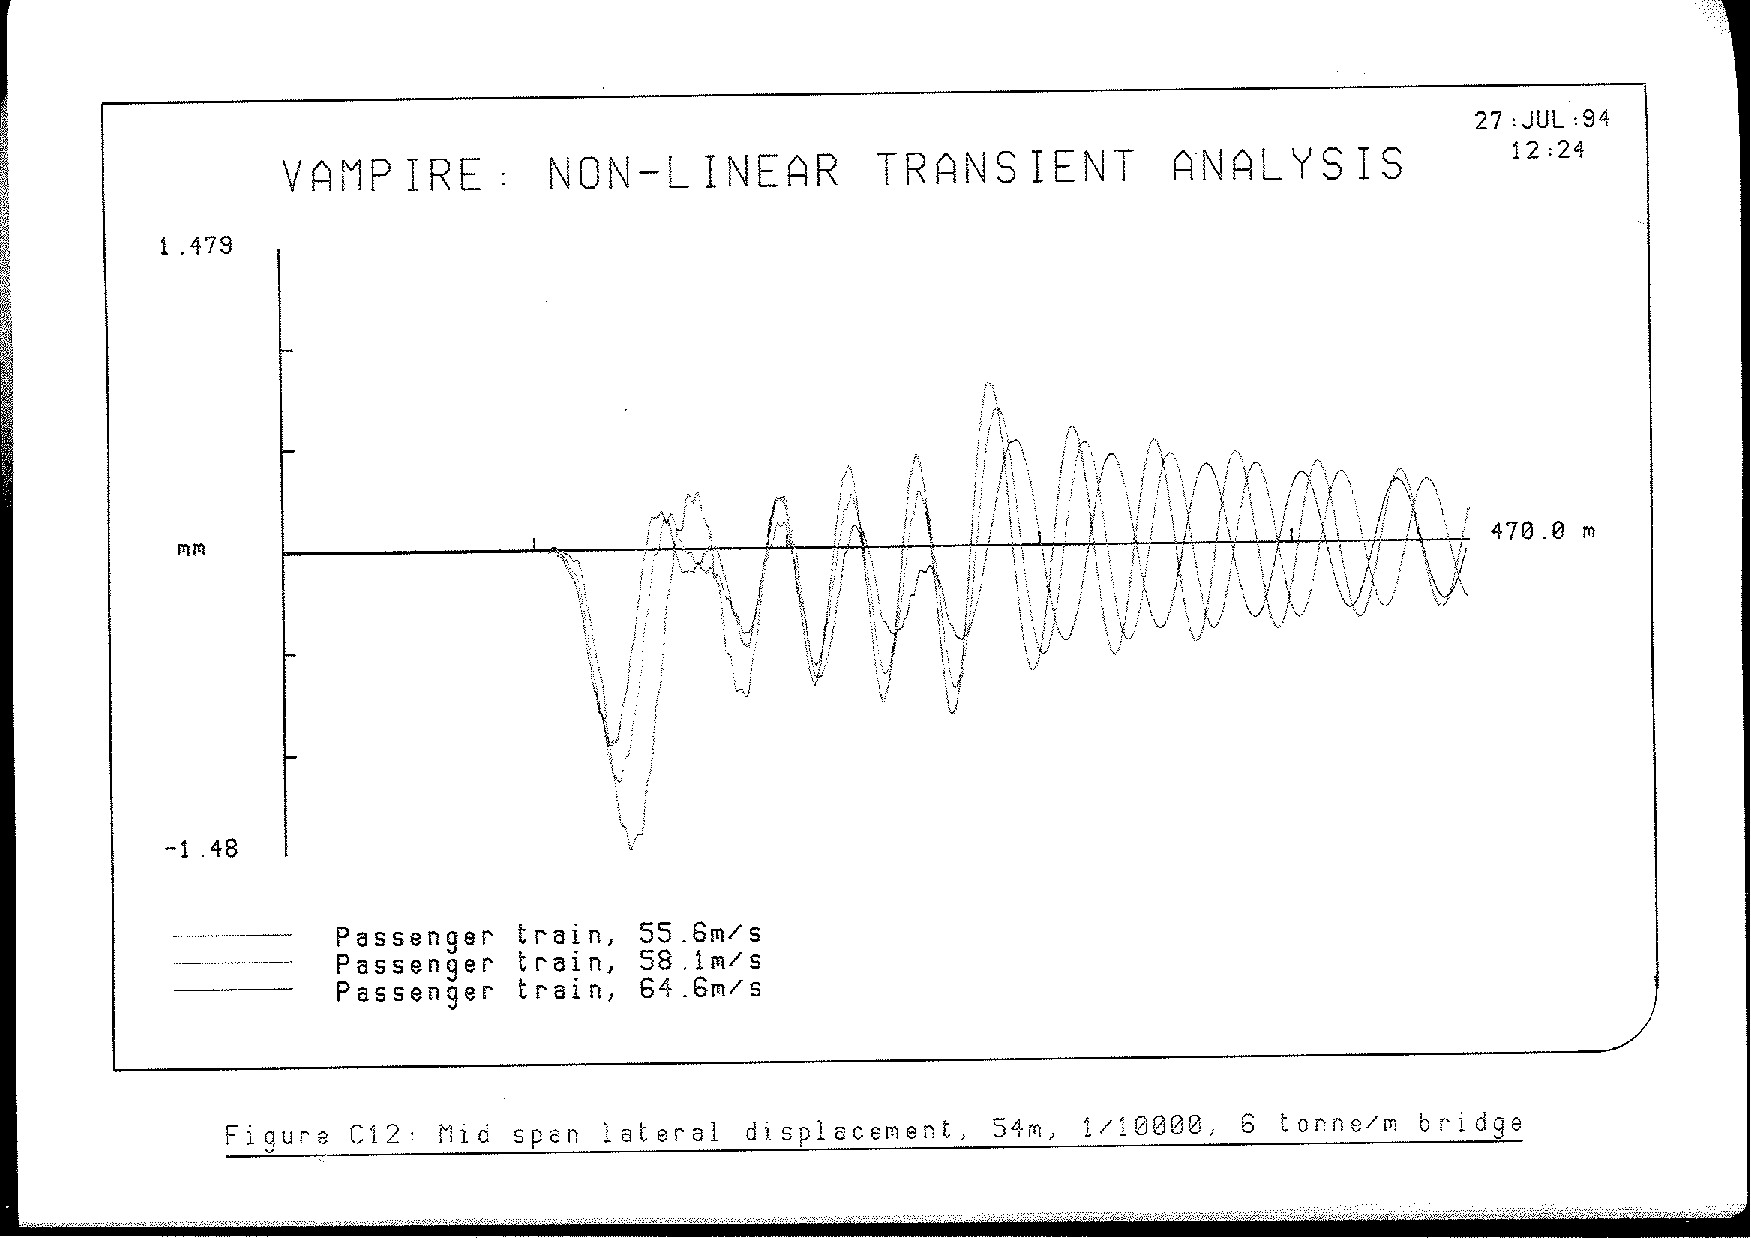
\includegraphics[width=0.8\textwidth]{c12}
    \caption{Figure C12 extracted from \citet{d181dt329} }
    \label{fig:c12}
\end{figure}

\begin{figure}[h!]
    \centering
    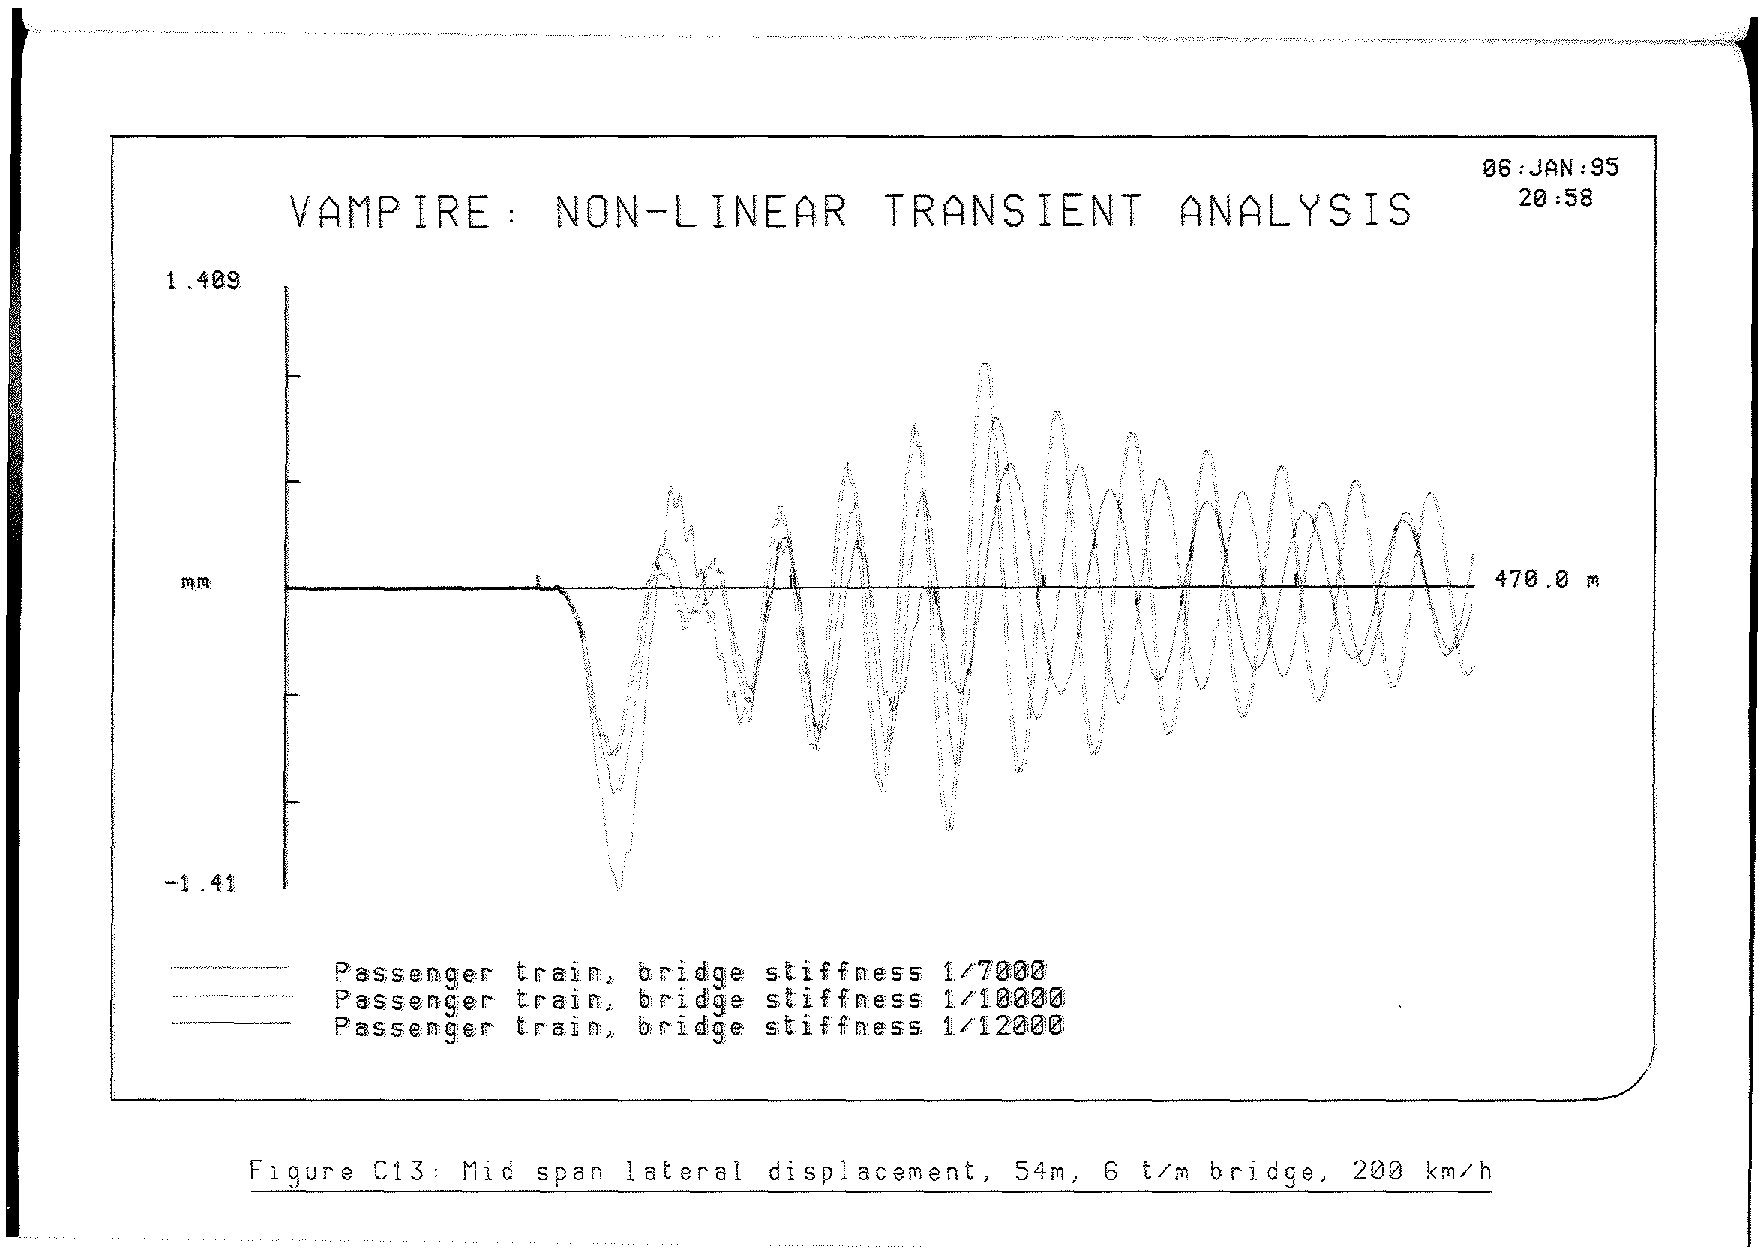
\includegraphics[width=0.8\textwidth]{c13}
    \caption{Figure C13 extracted from \citet{d181dt329} }
    \label{fig:c13}
\end{figure}

\begin{figure}[h!]
    \centering
    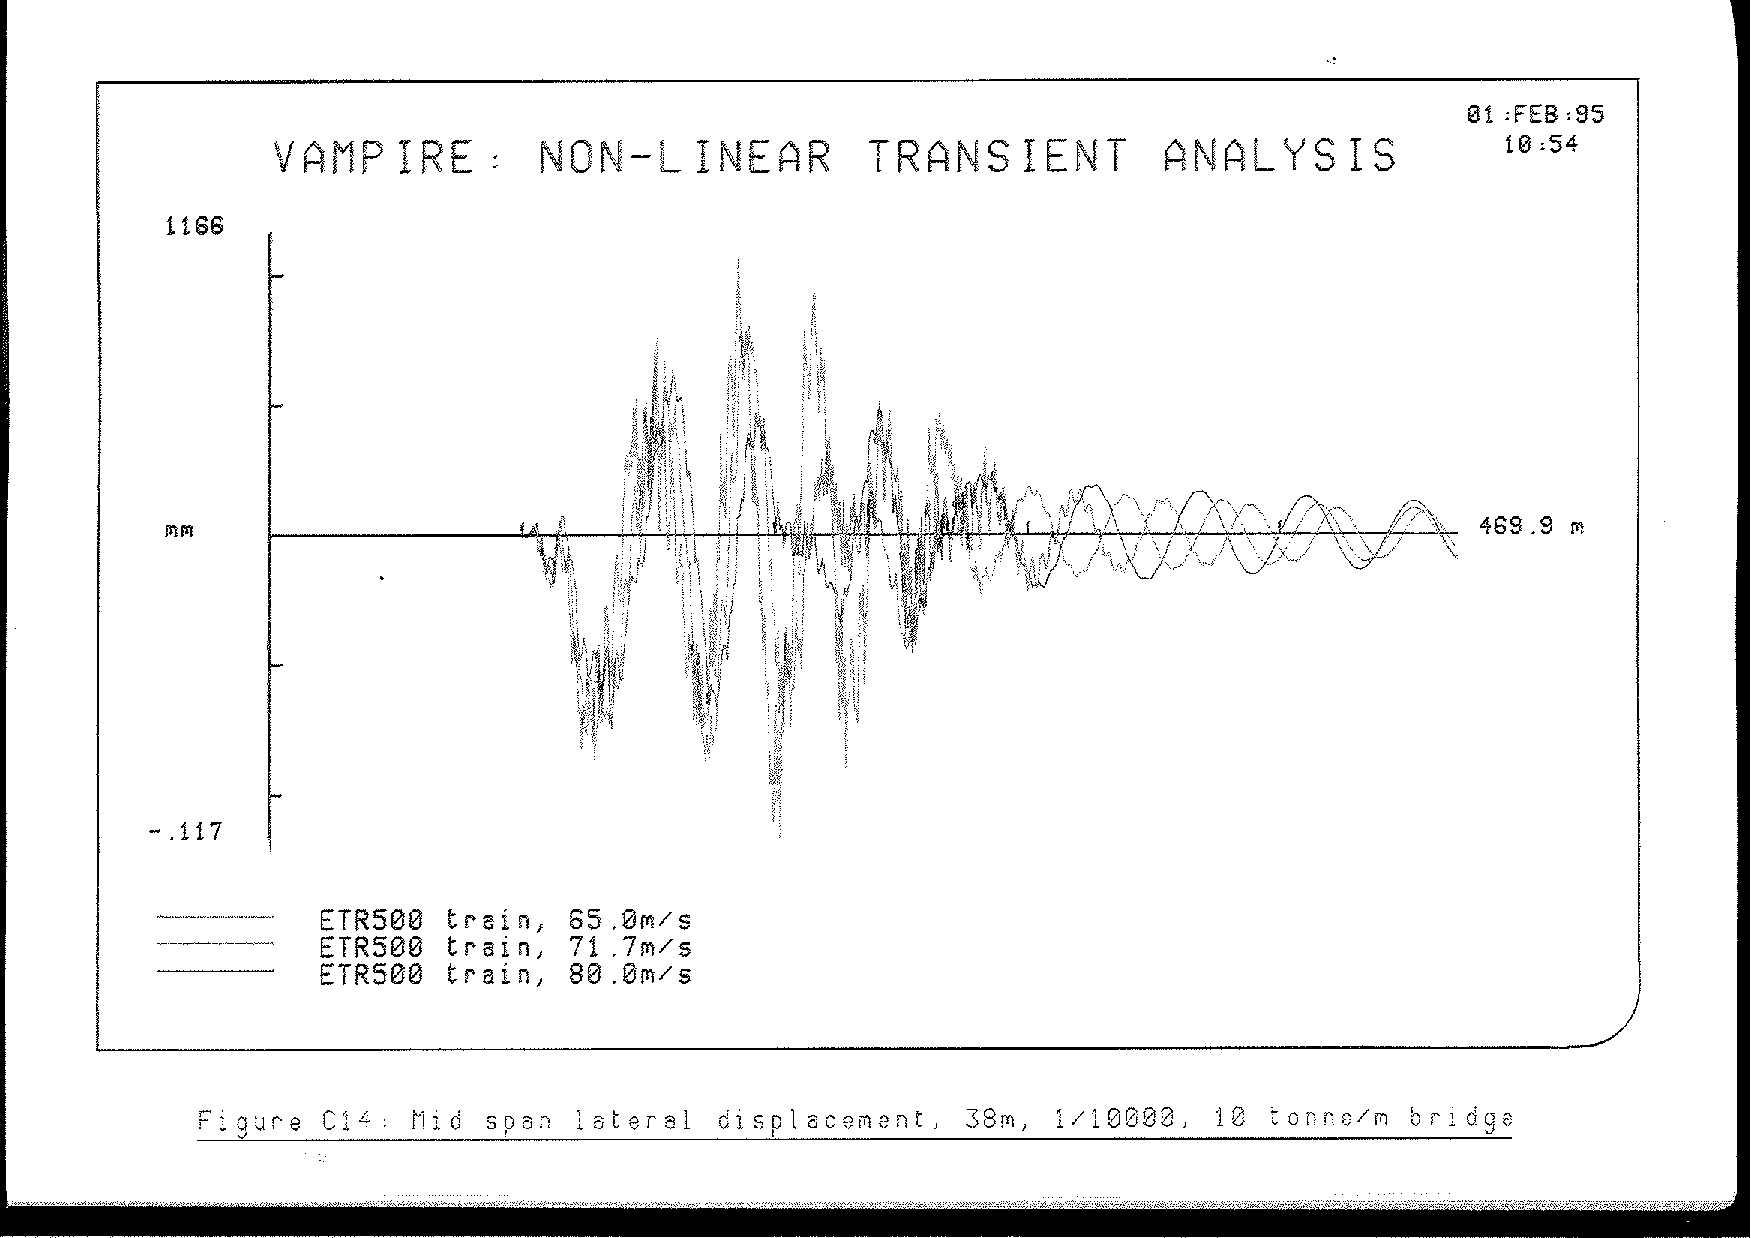
\includegraphics[width=0.8\textwidth]{c14}
    \caption{Figure C14 extracted from \citet{d181dt329}. An minor error is observed in y-axis label. Upper boundary of y-axis should be 0.116 }
    \label{fig:c14}
\end{figure}

To assure conservative comparison, only axle repeat pattern resonance results are selected because their output are more pronounced than kinematic resonance effect. Altogether 5 sets of reference data are selected. They include 2 reference data for freight trains(C3,C9), 2 reference data for passenger train(C12,C13) and 1 reference data for high-speed train(C14). Due to the fact that freight trains yield greater force than the other two types of trains, the analytical result should be conservative for the latter 3 cases. Since the output of C3 and C9 are already presented in Table.\ref{tab:parametersetupsandequivalentforce} so they are not being presented with other 3 sets of data this time. The bridge parameters and trains speed involved in these 3 cases(C12,C13,C14) are input into the analytical solution to yield analytical results.

\begin{table}[h!]
    \centering
    \caption{Comparison of results of simulation output and analytical output using refined load model}
    \begin{tabular}{c|ccc}
        \hline
         & C12 & C13 & C14\\
        \hline
        Stiffness($\sfrac{\delta_0}{t}$) & 1/10000 & 1/12000 & 1/10000\\
        Span($m$) & 54 & 54 & 38\\
        Mass per unit length($kg/m$) & 6000 & 6000 & 10000\\
        Speed of train($m/s$) & 55.6 & 55.6 & 65\\
        Damping ratio & 1\% & 1\% & 1\%\\
        Train type & Passenger & Passenger & High speed \\
        Track & Passenger Track & Passenger Track & High speed track\\
        \hline
        Peak Simulation displacement($mm$) & 1.48 & 1.41 & 0.117\\
        Peak Analytical displacement($mm$) & 6.6 & 5.8 & 3.0 \\
        \hline
    \end{tabular}
    \label{tab:comparisonresultssimulationanalytical}
\end{table}


In Table.\ref{tab:comparisonresultssimulationanalytical} the parameters involved in these 3 cases and their corresponding peak analytical results as well as peak simulation results are presented. 



\begin{figure}[h!]
\centering
\begin{tikzpicture}
\begin{axis}[
    symbolic x coords={C9,C1,C3,C12,C13,C14},
    xtick=data,
    legend style={at={(0.5,-0.15)},
        anchor=north,legend columns=-1},
    ybar=5pt,% configures `bar shift'
    bar width=9pt,
    nodes near coords,
]
\addplot 
    coordinates {(C9, 19.7) (C1, 14.5) (C3, 14.1)   (C12,6.6) (C13,5.8) 
        (C14, 3.0) };
\addplot 
    coordinates {(C9, 17.8) (C1, 14.2) (C3, 12.5)  (C12,1.48) (C13,1.41)
         (C14,0.117) };
\legend{Analytical peak displacement,VAMPIRE peak simulation displacement}
\end{axis}
\end{tikzpicture}
\caption{Comparison between VAMPIRE peak simulation result and analytical peak result}
\label{fig:comparisonpeaksimulationanalytical}
\end{figure}

To clearer illustrate the comparison of both peak results from simulation and analytical, Figure.\ref{fig:comparisonpeaksimulationanalytical} is created with rearranged x-axis order to make the descending trend more obvious. Please note all data sets except for C1 are valid for verification(C1 is used in creation of expression).

It can be seen that analytical results always keep a conservative margin above the simulation results. As expected, margins for C12,C13,C14 are bigger compared to C9,C1,C3 proofs that the analytical solution becomes more conservative if adopted to passenger train and high-speed train. What's more, the descending trend of analytical results follows the descending trend of simulation results perfectly regardless of train types. Thus considering these reasons, the analytical solution is sufficient for universal application on all train types.

\section{Equivalent load amplitude created using every other setup available}
Although the equivalent load amplitude using C1 as reference has been created, the result is not valid yet because C1 is equivalent to other 5 setup scenarios(C3,C9,C12,C13,C14). It is also necessary to carry out the same calculating process on other 5 setup scenarios.

Taking advantage of the process developed during the creation of C1 equivalent amplitude, the load equivalent amplitude of other 5 setups are calculated and then presented in the Table.\ref{tab:allLoadEquivalentAmplitude}.

\begin{table}[h!]
    \centering
    \caption{Load equivalent amplitude(N) from all available setups}
    \begin{tabular}{cccccc}
        \hline
        C1 & C3 & C9 & C12 & C13 & C14 \\
        \hline
        1928 & 1721 & 1760 & 427 & 463 & 228 \\
        \hline
    \end{tabular}
    \label{tab:allLoadEquivalentAmplitude}
\end{table}

Their corresponding benchmarks are presented in Table.\ref{tab:allBenchmark}.

\begin{table}[h!]
    \centering
    \caption{Benchmark on analytical peak displacement generated by all equivalent load amplitude by comparing simulation peak displacement}
    \begin{tabular}{ccccccc}
        \hline
        Analytical Peak Displacement & C1 & C3 & C9 & C12 & C13 & C14 \\
        \hline
        C1 & 0.0145 & 0.0141 & 0.0197 & 0.0066 & 0.0058 & 0.0003 \\
        C3 & 0.013 & 0.0125 & 0.0174 & 0.0059 & 0.0051 & 0.0036 \\
        C9 & 0.013 & 0.0128 & 0.0178 & 0.0061 & 0.0053 & 0.0032 \\
        C12 & 0.0032 & 0.0031 & 0.0043 & 0.00148 & 0.0013 & 0.0008 \\
        C13 & 0.0035 & 0.0034 & 0.0047 & 0.0016 & 0.00141 & 0.0002 \\
        C14 & 0.0021 & 0.0020 & 0.0028 & 0.0010 & 0.0008 & 0.00012 \\
        \hline
        Simulation Peak Displacement & 0.014 & 0.0125 & 0.0178 & 0.00148 & 0.00141 & 0.00012 \\
        \hline
        \label{tab:allBenchmark}
    \end{tabular}
\end{table}

Among all the equivalent load amplitude, the one created from C1 is most satisfying because its all outputs are conservative towards simulation output. Other equivalent load amplitude shows at least one nonconservative output. 

It can also be observed that the results of C12,C13,C14 are unacceptable due to the reason that their magnitude are too small. They can't predict reliable result for (C1,C3,C9). Their corresponding equivalent load amplitude will be ignored in the rest of the thesis.

Since there is few data available, it's meaningless to conduct further statistical procedures. The rest of the thesis will use the result of C1 because it's all conservative. However, the following section will give a simple guidance for statistical analysis provided by more simulations were done.

\section{Suggestions for further statistical analysis }

On the basis of more simulations could be conducted in the future, this section aims to give suggestions for further statistical analysis to improve the accuracy of the formula.

\paragraph{Filter out the influence of the parameters} It's essential to learn what roles are parameters playing in the simulation, so the simulations/analysis to be done should be planned ahead with a main objective which is  filtering out the influence on the bridge peak resonance displacement of the parameters such as bridge length, train speed, etc.

For example, by just looking at simulation peak displacement of C12,C13,C14, they are obviously small in magnitude compared to other 3. This is probably due to the reason that they all involve high speed train running. It could be that higher train speed tend to yield smaller deflection. However, this is only a hypothesis and needs more simulations to confirm.

\paragraph{Select correct statistical strategy} 

Content to be added after retrieving EN1990 Annex D.


\chapter{Finalizing the method for practical usage using real bridge parameters}

In practical usage, the speed that generates the highest peak response is unknown. Thus it is necessary to obtain the peak response for all speeds within the possible speed range. This is done by iterating the existing Matlab script with different speed. The increment in speed iteration is set in a way that ensures at least 1000 runs are done to guarantee precession. An example is illustrated as follows to show the usage on a real bridge project.

For an arch railway bridge located near Amsterdam, first step to is to collect following parameters:

$L = 255m$, $m = 5222e3kg$, $\mu = 2.0478e4 kg/m$, $EJ = 6.56e12Nm^2$

where:

$L$: span of the bridge

$\mu$: uniform mass per unit length of the bridge

$EJ$: lateral stiffness of the bridge

to test through a speed range of $1m/s - 30m/s$

Before beginning the calculation, make sure you have fog.m and Speedenvelop.m in your current working directory. By inputting following command in Matlab console, 

\texttt{Speedenvelop(6.56e12,255,2.0478e4,1,30,0.01)}


the envelop for displacement is generated and illustrated in Figure.\ref{fig:spedefEJ6560000000000L255min1max30mu20478.tikz}

\begin{figure}[h!]
\centering 
% \newlength\figureheight 
% \newlength\figurewidth 
\setlength\figureheight{6cm} 
\setlength\figurewidth{6cm} 
% This file was created by matlab2tikz v0.4.7 (commit 29117077607177efe915cc01d961cced006239c8) running on MATLAB 8.3.
% Copyright (c) 2008--2014, Nico Schlmer <nico.schloemer@gmail.com>
% All rights reserved.
% Minimal pgfplots version: 1.3
% 
\begin{tikzpicture}

\begin{axis}[%
width=\figurewidth,
height=\figureheight,
scale only axis,
xmin=0,
xmax=30,
ymin=0.0075,
ymax=0.011,
title={SpeedEnvelop def from1 to30}
]
\addplot [color=blue,solid,forget plot]
  table[row sep=crcr]{%
1	0.00781568842060085\\
1.2	0.00840892567977264\\
1.4	0.0088768875903958\\
1.6	0.00925769529057003\\
1.8	0.00957910144655464\\
2	0.00982648840148397\\
2.2	0.0100372557099215\\
2.4	0.0102060089657038\\
2.6	0.010347841028453\\
2.8	0.0104753362289414\\
3	0.010566090236029\\
3.2	0.0106426943938749\\
3.4	0.0107156879259678\\
3.6	0.0107656368912521\\
3.8	0.0108134770961416\\
4	0.0108433829006734\\
4.2	0.0108762461970553\\
4.4	0.0109009754438711\\
4.6	0.0109137058875431\\
4.8	0.0109063964703489\\
5	0.0109283926778865\\
5.2	0.0109354115709882\\
5.4	0.010934364378216\\
5.6	0.010925358882146\\
5.8	0.0109155184260617\\
6	0.0109160952245694\\
6.2	0.0109022893020932\\
6.4	0.0108894990281659\\
6.6	0.0108791296950589\\
6.8	0.0108683159097076\\
7	0.0108485530748728\\
7.2	0.0108354499334163\\
7.4	0.0108143121429067\\
7.6	0.0107967054438007\\
7.8	0.0107826189027167\\
8	0.0107571129205081\\
8.2	0.0107450192698353\\
8.4	0.0107182431373167\\
8.6	0.0107081009100856\\
8.8	0.0106810097968274\\
9	0.0106647893596357\\
9.2	0.0106368269751327\\
9.4	0.0106244435627288\\
9.6	0.0105902161380316\\
9.8	0.0105787489298167\\
10	0.0105530497685275\\
10.2	0.0105311301588914\\
10.4	0.0105155111529359\\
10.6	0.0104818416711415\\
10.8	0.0104658192794055\\
11	0.0104515232844051\\
11.2	0.0104195968460413\\
11.4	0.0103992383576141\\
11.6	0.0103875827376142\\
11.8	0.0103585518798102\\
12	0.0103282987036047\\
12.2	0.0103183620397562\\
12.4	0.0103012474040927\\
12.6	0.0102668977746374\\
12.8	0.0102449204320541\\
13	0.0102354809790005\\
13.2	0.0102169579397151\\
13.4	0.0101865143682396\\
13.6	0.0101530378665145\\
13.8	0.0101488592884028\\
14	0.0101342026283539\\
14.2	0.0101129828210581\\
14.4	0.0100781640001081\\
14.6	0.010051230942275\\
14.8	0.0100463931273211\\
15	0.0100339102223161\\
15.2	0.0100154789040376\\
15.4	0.00998674150551577\\
15.6	0.00995047989615967\\
15.8	0.00993544019804088\\
16	0.00993088834100722\\
16.2	0.0099199018939231\\
16.4	0.00990104705345698\\
16.6	0.00987441551082942\\
16.8	0.00984237739719204\\
17	0.00980928040956712\\
17.2	0.0098093242438416\\
17.4	0.00980329783311577\\
17.6	0.00979122702961792\\
17.8	0.00977314390458511\\
18	0.00974908670711774\\
18.2	0.00972108217302529\\
18.4	0.0096776691907686\\
18.6	0.00966812567615805\\
18.8	0.0096672743699076\\
19	0.00966167442250244\\
19.2	0.00965133478148734\\
19.4	0.00963626874305325\\
19.6	0.00961649393213872\\
19.8	0.00959203227865456\\
20	0.00956290998985286\\
20.2	0.0095021185042862\\
20.4	0.00950695108828918\\
20.6	0.00950797086177456\\
20.8	0.00950518266938973\\
21	0.00949859410737403\\
21.2	0.00948821551471712\\
21.4	0.00947405996230233\\
21.6	0.00945635016311157\\
21.8	0.00943490732597904\\
22	0.00940971735699768\\
22.2	0.00931048059107463\\
22.4	0.00931929357671497\\
22.6	0.00932536783564737\\
22.8	0.00932827887006457\\
23	0.00932803971339443\\
23.2	0.00932466491318731\\
23.4	0.00931817052503146\\
23.6	0.00930857410555171\\
23.8	0.00929589470449585\\
24	0.0092803683442182\\
24.2	0.00926243390849551\\
24.4	0.0092414380792758\\
24.6	0.00916278336234724\\
24.8	0.00909609061802426\\
25	0.00910564521095271\\
25.2	0.00911382028447303\\
25.4	0.00911959836984988\\
25.6	0.00912274595493189\\
25.8	0.00912328389307619\\
26	0.00912136767440461\\
26.2	0.00911807810466714\\
26.4	0.00911219402539695\\
26.6	0.00910373969614448\\
26.8	0.0090927400294876\\
27	0.00907945686157787\\
27.2	0.00906461860626204\\
27.4	0.00904726523290454\\
27.6	0.00902380873477224\\
27.8	0.00882644457839617\\
28	0.00883996385182427\\
28.2	0.00885231633946435\\
28.4	0.00886244919403873\\
28.6	0.00887051931610704\\
28.8	0.00887784576510649\\
29	0.0088829756466977\\
29.2	0.00888593368675971\\
29.4	0.00888785865101469\\
29.6	0.00888798738354364\\
29.8	0.00888597303168551\\
30	0.00888235391855735\\
};
\end{axis}
\end{tikzpicture}% 
\caption{Peak deflection at mid-span with regard to changing train speed. Parameters: $EJ = 6.56e12Nm^2$, $L= 255m$,$\mu = 20478 kg/m$, $c_{min}=1m/s$, $c_{max} = 30m/s$} 
\label{fig:spedefEJ6560000000000L255min1max30mu20478.tikz} 
\end{figure}

The plot shows that the critical speed appears at approximately $5m/s$ and corresponding peak deflection response is approximately $11mm$. 

Since the relationship between end support rotation angle and mid-span deflection is widely known as:

$$ \varphi = \frac{3}{L}\cdot \delta_0  $$

and rotation is yielded as:

$$ \varphi = \frac{3}{255}\times 0.011 = 0.00013 $$

This value is much lower than the rotation value regulated in EN1991-2. See Section.\ref{sec:Transverse-deformations-and-vibrations} for criteria details.

Thus the conclusion can be made that this bridge is safe subjected to lateral dynamic load.

However, if encountering unfavourable peak result, a filter can be applied on the train speed to further cut off the peak response. In previous chapter it has been already be concluded that all resonance effects between train and bridge are wavelength phenomenon. In order to couple frequency with bridge's first natural bending frequency, the train needs to operate at a certain speed range. 

For example, according to Chapter.\ref{sec:wavelengthstudy}, the possible wavelength range for trains in the Netherlands is approximately 10m-30m, including both axle repeat wavelength and kinematic wavelength. 

The natural frequency of the bridge in this example is 

$$ f_1 = \frac{\pi}{2l^2}\sqrt{\frac{EJ}{\mu}} = \frac{\pi}{2\times 255^2}\sqrt{\frac{6.56e12}{1.0478e4}} = 0.4Hz$$

so the possible resonance speedis obtained by multiplying wavelength range with natural frequency, yielding: $4m/s$ and $12m/s$

Although this speed filtering range doesn't help to cut off maximum response in this case because critical speed stills remains in the speed range, the filter can be more effective for bridges possessing higher first natural frequency simply because both lower and upper boundary for speed filtering range is linear to beam's first natural frequency. While it's not likely for upper boundary to shift to the left side of the critical speed, it's more favourable for lower boundary to shift to the right side of the critical speed.

\section{Conclusion}

The new practical method for checking lateral resonance response of railway bridge is developed in this chapter. This method is capable to simulate a resonance scenario where the bridge was passed by a moving railway vehicle. 

The method shows conservative prediction compared to VAMPIRE simulations. However, since lack of data can be used to further verify the practical method, results on longer span bridges can not be verified until new simulations or measurements data are obtained.

A general conclusion in finalizing phase of practical method is, for a certain bridge, faster train speed doesn't necessary cause higher resonance response of the bridge. As can be seen in Figure.\ref{fig:spedefEJ6560000000000L255min1max30mu20478.tikz}, critical speed appears at approximately $5m/s$, and response start to fall when speed is higher than $5m/s$. This means comparing to higher load amplitude caused by higher train speed, the shorter loading time caused by same reason is more dominating. By considering the fact in Figure.\ref{fig:comparisonpeaksimulationanalytical} that the analytical is even more conservative for higher speed, it can be concluded than high-speed trains cause less dynamic problem for lateral bridge dynamics.

Matlab scripts are already written and attached for the convenience of readers. Since the explicit solution has been given in the chapter, it's completely possible to adopt them in other mathematical software for different preferences.

\chapter{Conclusion}


Two proposed criteria in RP6\citet{d181} were adopted in Eurocode 1991-2. One of them is 1.2Hz criterion. It was adopted without amending. The other one is lateral force models. Loading models were adopted in a different name as 'nosing force' in \citet[A6.5.2]{EC12}. 

\begin{enumerate}[-]
\item The 1.2Hz criterion was aiming to avoid the occurrence of resonance between bridge first lateral vibration mode and vehicle sway mode, however, no research can be found among all D181 report series to support this hypothesis. This criterion was proposed without a valid background.

\item Nosing force in EN1991-2 has a single characteristic value of 100kN, while RP6 proposes different values for different scenarios. Also, it is proved that nosing force isn't conservative when resonance happens between the vehicle and the bridge.
\end{enumerate}

In addition, D181 did research on other 2 resonance phenomenons, including axle repeat pattern resonance and kinematic movement resonance. Resonance was proofed to be possible and was successfully reproduced using VAMPIRE software. These two resonance are wavelength phenomenon, meaning resonance can happen on any train/bridge combination.

However, the dynamic effects start to build up at a broader frequency, which means even if the resonance is avoided between bridge and train, the response of the bridge will still be amplified by dynamic loading. The relationship between total peak lateral force of the first two traction units and speed is found by using the simulation output and regression approach. The lateral force is greatly dependant on track quality, train type and speed.

Nosing force model was proposed by investigating the peak lateral force on track with a standard deviation of 7mm. Such track irregularities ensures the occurrence of hunting effects thus this value is conservative. However, for tracks maintained as regulation requires, up to 2mm standard deviation is allowed. Since track force increases as track standard deviation does, it can be concluded that 100kN of characteristic value for nosing force is very conservative.

By using the knowledge above, a practical method for easy calculating real-time mid-span resonance responses of the bridge is also developed. The method features a analytical model and an equivalent amplitude model. The equivalent amplitude model is developed based on both the simulation result of VAMPIRE software and the relationship between lateral force and train speed discovered earlier in the report. The practical method shows reasonable conservative prediction when compared to other reference data in DT329 reports.

However, as VAMPIRE simulation results only have span up to 120m, there’s no benchmark can be found to validate the correctness of the formula for longer span inputs. So it is highly advisable that more simulations/measurements to be done to verify the correctness of result for longer span bridges.

\chapter{Recommandations on future reseraches}

Future reseaches to be proposed in this section are mainly related to heavy FEM transient analysis. Although D181 commiittee conducted a number of simulations in D181 report seriers, the response of longer span bridges remaines unknown. What's more, D181 report series were created in 1990's. The trains and their parameters used in the report are too old for nowadays usage.

The aim of proposed FEM simulations is to verify the practical method described in this thesis. The method is needed to be verified for longer span bridges and modern vehicle design. As a conclusion, simulations with following objectives are needed to be done:

\begin{enumerate}
    \item Lateral forces on tracks of modern vehicles/tracks
    \item Resonance response of bridges with span longer than 150m
\end{enumerate}

These simulations should be done with following extra requirements on the basis of simulations done in resonance study of DT329:

\begin{enumerate}
    \item More realistic and up-to-date data on modern train vehicles
    \item More realistic data on lateral track irregularities
    \item Broader range of bridge span to be investigated(greater than 150m)
\end{enumerate}

More accurate statistical result can be yielded with more simulation data. Since now only 6 sets of data can be used, the new practical method can hardly be globally reliable. However, it is recommended that future research uses a larger simulation data base to further improve the accuracy of the new method.

Transient simulations of this topic is very resource demanding. It is impossible for this thesis to carry out these simulations. Thus above simulations are proposed to whoever poceesing the resource and willingness to further investigate the topic. It is also proposed that lateral force data caused by running trains to be evaluated more frequently.

The practical method should be verified by comparing its own result with result of newly conducted simulations. The result of practical method should be conservative according to the comparison. 

It is possible to modify the amplitude in practical method to a less conservative value according to newly conducted simulations. It is expected that newly conducted simulations yield smaller lateral force on tracks because of the advanced suspension systems implemented in modern vehicle designs and better track quality.